\documentclass{standalone}

\usepackage{tikz}
    \usetikzlibrary{arrows.meta}

\usepackage{graphicx} % Работа с графикой \includegraphics{}
\graphicspath{{./images/img1/}} % картинки в папке ./images/img1/
    
\begin{document}

\begin{tikzpicture}
    \node  at (0,0) 
        {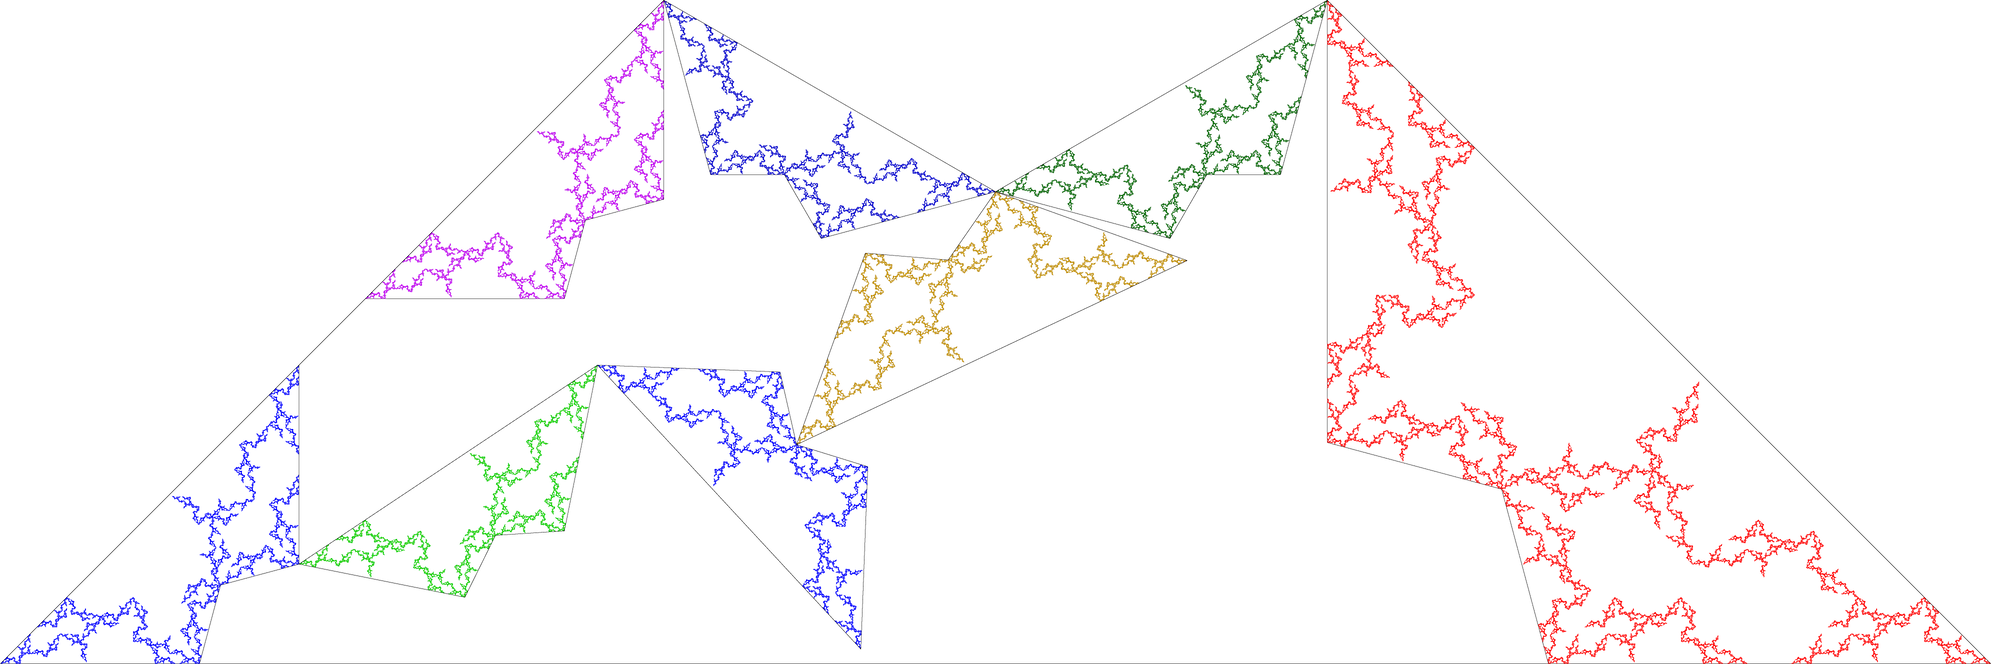
\includegraphics[width=11.9cm]{ex.png}};
    %\draw[help lines] (-6,-2) grid (11,2);
    \node[shape=circle, draw, line width=1pt] 
        (k3) at (7.7,0) {$3$};
    \node[shape=circle, draw, line width=1pt, red] 
        (k1) at (10.7,-1.7) {$1$};
    \node[shape=circle, draw, line width=1pt] 
        (k4) at (5.5,0) {$5$};
    \node[shape=circle, draw, line width=1pt, red] 
        (k2) at (10.7,1.7) {$2$};
    \node[shape=circle, draw, line width=1pt] 
        (k5) at (9,0) {$4$};
    \path[->,>={Latex[length=7pt]},line width=1pt] 
        (k1) edge[red,thick,bend right=25] node[left, black]{$1$} (k2)
        (k2) edge[red,thick,bend right=25] node[right, black]{$6$} (k1)
        (k4) edge[bend right=15] node[below]{$2$} (k1)
             edge[bend left=15] node[above]{$3$} (k2)
             edge node[above]{$5$} (k3)
        (k3) edge[bend left=7] node[above]{$6$} (k2) 
             edge[bend right=7] node[below]{$4$} (k1)
        (k5) edge node[above]{$3$} (k1) 
             edge node[below]{$4$} (k2);
    \fill[black] (-5.95,-1.95)
         circle (0.07) 
         node[left=1mm] {\large$1$};
    \fill[black] (5.95,-1.95)
         circle (0.07) 
         node[right=1mm] {\large$2$};
    \fill[black] (1.97,2)
         circle (0.07) 
         node[above=1mm] {\large$3$};
    \fill[black] (-1.97,2)
         circle (0.07) 
         node[above=1mm] {\large$4$};
    \fill[black] (0,0.85)
         circle (0.07) 
         node[above=1mm] {\large$5$};
    \node at(-5.2,-0.8){$P_1$};
    \node at(-3.2,1.2){$P_2$};
    \node at(-0.9,1.6){$P_3$};
    \node at(0.9,1.6){$P_4$};
    \node at(0.2,-0.3){$P_5$};
    \node at(2.7,-1.3){$P_6$};
\end{tikzpicture}

\end{document}